\section{Theorie}
\label{sec:Theorie}
Die Dotierung von einwertigen Ionengittern mit zweiwertigen Kationen verursacht elektrische Dipole.
Da ein Kristall nach außen hin ladungsneutral ist, entstehen Leerstellen. Diese Leerstellen und die zweiwertigen
Kationen bilden die Dipole. Die Verbindungsachse zwischen diesen Störstellen legt die Orientierungsrichtung
fest. Dieser Sachverhalt ist in Abbildung \ref{fig:kristall} dargestellt.
\begin{figure}
    \centering
    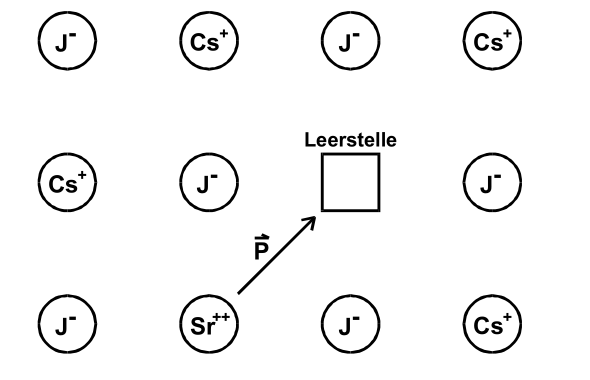
\includegraphics[width=0.5\textwidth]{kristall.PNG}
    \caption{Dipol im Kristallgitter.\cite{skript}}
    \label{fig:kristall}
\end{figure}\\
Unter dem Einfluss eines elektrischen Feldes bei Temperaturen unter $500\ \si{\celsius}$ können die Dipole
sich nur durch Leerstellendiffusion ausrichten. Allgemein sind die Ausrichtungen diskret, da die Störstellen
nur auf Gitterpunkten liegen können. Damit eine Dipolausrichtung stattfindet muss eine Aktivierungsenergie
zur Überwindung einer Potentialbarriere zugeführt werden.
Die Form der Potentialbarriere ist materialspezifisch und festgelegt durch den räumlichen und periodischen
Verlauf des Gitterpotentials. Die Zeit zwischen zwei Ausrichtungen wird Relaxationszeit genannt und hängt über
die Relaxationsgleichung mit der Aktivierungsenergie $W$ zusammen:
\begin{align}
 \tau(T) =\tau_\mathrm{0}\exp\left({\frac{W}{kT}}\right) \label{eqn:relaxationsgleichung}\text{,}
\end{align}
mit $\tau_\mathrm{0}$ als charakterischtische Relaxationszeit.

Der Anteil der in einem elektrischen Feld ausgelenkten Dipole wird durch die Langevin-Gleichung beschrieben:
\begin{align}
  y=L(x)&=\cothx{x}-\frac{1}{x}   &\text{mit}\,\, x=\frac{pE}{kT};
\end{align}
Hierbei ist $p$ der Betrag des Dipolmomentes. Unter der Annahme, dass $pE<<kT$ lässt sich der Ausdruck
für den Anteil der ausgerichteten Dipole ausdrücken als:
\begin{equation}
  y(T)=\frac{pE}{3kT}.
\end{equation}
Bei der Umorientierung der Dipole kann ein sogenannter Dipolarisationsstrom gemessen werden, der Verlauf
ist in Abbildung \ref{fig:strom} dargestellt.
\begin{figure}
    \centering
    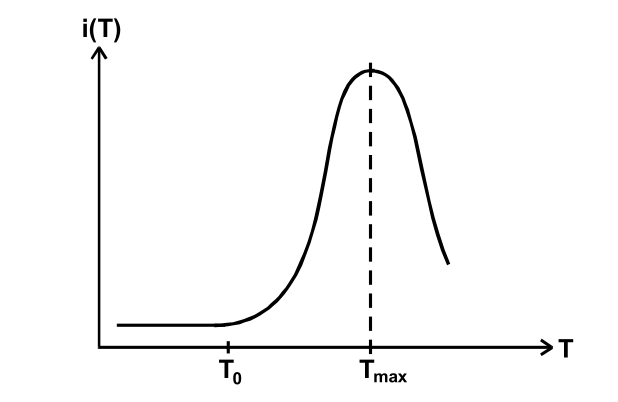
\includegraphics[width=0.7\textwidth]{strom.PNG}
    \caption{Verlauf vom Dipolarisationsstrom in Abhängigkeit von der Temperatur.\cite{skript}}
    \label{fig:strom}
\end{figure}
Hierbei beschreibt $T_\mathrm{0}$ den Startpunkt der Relaxation und das
Tupel $T_\matrhm{max}$ und $I(T_\mathrm(max))$ den maximalen Dipolarisationsstrrom.
Der rasche Anstieg zu Beginn kann mit der schnell abnehmenden Relaxationszeit erklärt werden,
der anschließende Abfall durch die immer geringer werdende Anzahl an noch nicht relaxierten Dipolen.
Es kann eine Dipolarisationsstromdichte definiert werden:
\begin{equation}
  j(T)=y(T)p\frac{\mathrm{d}N}{\mathrm{d}t}\label{eqn:stromdichte}.
\end{equation}
Diese besteht aus dem Produkt von $p$, dem Dipolmoment, dem
Anteil der Dipole und $\frac{dN}{dt}$
die Anzahl der relaxierenden Dipole pro Zeit und Volumeneinheit.
Für $py(T)$ gilt:
\begin{equation}
py(T)=\frac{p^2E}{3kT_\mathrm{p}}.\label{eqn:prod}
\end{equation}
Die Anzahl der relaxierenden Dipole $\frac{dN}{dt}$ lässt sich auch als Zahl $N$ der zum Zeitpunkt $t$ pro Volumeneinheit orientierten Dipole
darstellen, da es sich hier um einen thermisch aktivierten Prozess handelt.
Mit der Relaxationsfrequenz $\frac{1}{\tau}$ als Proportionalitätsfaktor gilt:
\begin{equation}
  \frac{\mathrm{d}N}{\mathrm{d}t}=-\frac{N}{\tau(T)}\label{eqn:dgl}.
\end{equation}
Diese Differentialgleichung lässt sich lösen mit:
\begin{equation}
  N= N_\mathrm{p}\exp\left({-\frac{1}{b}\int_{T_\mathrm{0}}^{T} \frac{\mathrm{d}T'}{\tau(T')}}\right)\label{eqn:loesung}.
\end{equation}
Hierbei ist $N_\mathrm{p}$ die Anzahl der zu Begin einer Aufheizung orientierten Dipole und
$b$ eine Heizrate. Mit den Gleichungen \eqref{eqn:stromdichte} bis \eqref{eqn:loesung}
und der Relaxationsgleichung \eqref{eqn:relaxationsgleichung} folgt für die Stromdichte:
\begin{equation}
j(T)=\frac{p^2EN_\mathrm{p}}{3kT_\mathrm{p}\tau_{0}}\exp\left(-\frac{1}{b\tau_\mathrm{0}}\int_{T_\mathrm{0}}^{T}\exp\left(\frac{-W}{kT'}\right)\mathrm{d}T'\right)\exp\left(\frac{-W}{kt}\right). \label{eqn:8}
\end{equation}
